\chapter{Implemented Algorithms}
\label{cha:implementedAlgorithms}


%---------------------------------------------------------------------------

\section{Trend following}
\label{trend_following_impl}

The crux of the trend following method is to choose a set of entry and exit point conditions that determine our \emph{trading strategy} (predefined set of rules 
responsible for making buy/sell decisions).
Simple Moving Average (SMA) is especially useful to highlight longer-term trends in a set of data points.

SMA is formulated as the unweighted mean of the previous $N$ data points:

\begin{equation}
    SMA_{today,N} = \frac{\sum_{i=1}^{N}p_{today - i}}{N}
\end{equation}

\begin{description}
  \item [$p_{j}$] 
    value of data on day $j$
\end{description}

In this case, data points will represent closing stock prices. 
 


\textbf{Entry points:}
  \begin{itemize}
    \item Simple moving average (SMA) of last $N$ days is greater than SMA of last $M$ days ($N$ < $M$)
    \item Current stock price is max of last $N$ days (that is usually a good indicator of lucrative opportunity on the market)
  \end{itemize}

As soon as at least one of the above conditions is satisfied we go long (we buy a particular asset).


\textbf{Exit points:}
  \begin{itemize}
    \item Losses on a single trade are greater than 2 \% (this rule is used to quickly abandon an investment that we were wrong about its trend direction,
	  the amount of tolerable loss solely depends on our strategy and does not have to be exactly 2\%)
    \item Simple moving average (SMA) of last $N$ days is lesser than SMA of last $M$ days ($N$ < $M$)
  \end{itemize}

As soon as the exit condition is satisfied we go short (we sell a particular asset).
 
Obviously the above rules are very simple and quite straightforward.
Nonetheless, the system based on them proves to be robust, as shown in chapter \ref{cha:tests}.
   
By manipulating the value of $N$ we can seek out different types of trends, as mentioned in \ref{sec:types_of_trends}. 

\subsection{Pseudocode}

Algorithm~\ref{fig:tf_pseudo} shows pseudocode of trend following.


\begin{description}


\item[SMA(i,N)]
  calculates Simple Moving Average for stock $i$, $N$ last days are taken into account  
\item[go\_short(i)]
  sell stock $i$
\item[go\_long(i)]
  buy stock $i$
\item[get\_current\_stock\_price(i, day)]
  returns stock $i$ price for specific $day$ 
\item[get\_most\_recent\_trade\_price(i)]
  returns the price we paid for stock $i$ (we have stock $i$ in our portfolio)
\item[max(i,N)]
  returns the maximum price for stock $i$ in the last $N$ days
\item[N, M, maximal\_value\_loss]
  modifiable parameters
\end{description}
% 


% \begin{algorithmic}
% 
% \STATE $maximal\_value\_loss \gets 0.98$
% 
% \FOR{$day = 1$ to $max\_day$} 
% 
%   \FOR{$i = 1$ to $number\_of\_stocks$}
% 
%     \IF {$ get\_most\_recent\_trade\_price(i) < maximal\_value\_loss * get\_current\_stock\_price(i, day) $} 
% 	    \STATE $go\_short(i)$
%     \ELSE
% 	    \IF {$SMA(i,N) < SMA(i,M)$}
% 		    \STATE $go\_short(i)$
% 	    \ENDIF
%     \ENDIF
% 
%     \IF {$SMA(i,N) > SMA(i,M)$} 
% 	    \STATE $go\_long(i)$
%     \ELSE
% 	    \IF {$max(i,N)) <= get\_current\_stock\_price(i, day)$}
% 		    \STATE $go\_long(i)$
% 	    \ENDIF
%     \ENDIF
% 
%   \ENDFOR
% 
% \ENDFOR
% 
% \end{algorithmic}

\begin{algorithm}
  \SetKwData{parents}{parents}
  \SetKwData{maxDays}{maxDays}
  \SetKwData{numberOfStocks}{numberOfStocks}
  \SetKwData{maximumValueLoss}{maximumValueLoss}
 
  \SetKwFunction{SMA}{SMA}
  \SetKwFunction{getMaxStockPrice}{getMaxStockPrice}
  \SetKwFunction{goShort}{goShort}
  \SetKwFunction{goLong}{goLong}
  \SetKwFunction{getMostRecentTradePrice}{getMostRecentTradePrice}
  \SetKwFunction{getCurrentStockPrice}{getCurrentStockPrice}
  \SetKwFunction{mutateLeastFitIndividuals}{mutateLeastFitIndividuals}
  \SetKwFunction{extinctLeastFitIndividuals}{extinctLeastFitIndividuals}
  \SetKwInOut{Input}{input}\SetKwInOut{Output}{output}
 
  \Input{$N$, $M$}
  \BlankLine
  \maximumValueLoss $\leftarrow$ 0.98 \;
  
  \For{$day\leftarrow 1$ \KwTo \maxDays}{

     \For{$i\leftarrow 1$ \KwTo \numberOfStocks}{
      
      \BlankLine

	\If(){\getMostRecentTradePrice{$i$} < \maximumValueLoss * \getCurrentStockPrice{$i$, $day$} }{
	  \goShort{$i$} \;
      }
      \ElseIf{\SMA{$i$, $N$} < \SMA{$i$, $M$}}{
	   \goShort{$i$} \;
	}

      \BlankLine

      \If(){\SMA{$i$, $N$} > \SMA{$i$, $M$} }{
	  \goLong{$i$} \;
      }
      \ElseIf{\getMaxStockPrice{$i$, $N$} <= \getCurrentStockPrice{$i$, $day$} }{
	   \goLong{$i$} \;
	}


    }
  }
  \caption{Trend following pseudocode}\label{fig:tf_pseudo}
\end{algorithm}



\subsection{R}

R is a programming language designed to deal with building systems based on statistical computation.
Apart from that it offers command line interpreter.
Working with vectors and matrices of data is straightforward and robust.
Its high performance and vast library of already implemented statistical functions are the main advantages of R (\cite{R}).    

\section{Genetic algorithm}
\label{sec:genAlgoImpl}

\subsection{Adjusting GA to solve portfolio optimization problem}

As described in \ref{sec:genAlgorithms} each potential solution shoul be encoded inside a chromosome. 
Each chromosome represents portfolio composition (it is a normalized vector of double values representing percentage share of each stock).
Before first round of computation, the entire population is created from scratch using random values in chromosomes.

The following modified GA operations have been implemented:
\begin{description}
  \item [mutation]
      Mutation operator changes exactly one value $ \alpha_{i} $ representing percentage share of a specific stock $i$ (each time the value $i$ is chosen randomly)
      to $\alpha_{i}'$ ($\alpha_{i}' \in (0,1)$ is chosen randomly). 
      After that, we have to normalize vector.
      \emph{Mutation\_coefficient} (\emph{mutation\_coefficient} $ \in (0,1)$ ) determines what part of population will be subjected to mutation operator.
  \item [selection]
      \emph{breeding\_coefficient} ( \emph{breeding\_coefficient} $ \in (0,1)$ ) determines what part of population will be subjected to crossover operator, selection is based on 
      fitness function (only the fittest part of the population will be selected)
  \item [crossover]
      After selection chromosomes eligible for reproduction, each pair of chromosomes are subjected to crossover operator. As a result new chromosomes are created (each pair
      produces two new chromosomes) and added to population. Crossover choose points $left$  and $right$ (both are chosen randomly) which cut parent's chromosomes in the following
      way: 
	  \begin{figure}[H]
	    \begin{center}
	      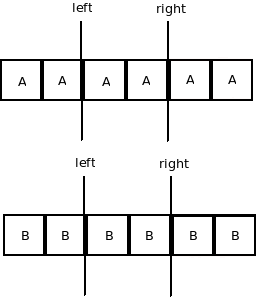
\includegraphics[scale=.4]{parents.png}
	    \end{center}
	    \caption{Example of parent's chromosomes split into 3 parts}
	  \end{figure}

	Now children are created in the following way:    
	  \begin{figure}[H]
	    \begin{center}
	      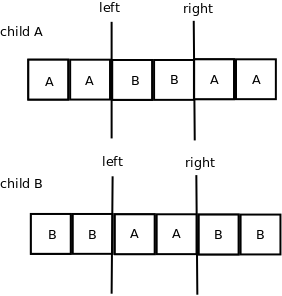
\includegraphics[scale=.4]{children.png}
	    \end{center}
	    \caption{Children's chromosomes contain mixed parent's genetic material}
	  \end{figure}

\end{description}

Apart from that, extinction mechanism has been implemented.
At the end of each GA round a part of the population that has the lowest fitness is exterminated.
\emph{Extinction\_coefficient} determines what part of population will be subjected to extinction.
 
\subsection{Pseudocode}

% \begin{algorithmic}
% 
% \STATE randomly INITIALISE the $population$ 
% \FORALL{ $day$ }
%   \STATE EVALUATE each individual
%   \STATE SELECT parents
%   \STATE RECOMBINE pairs of parents to create offspring
%   \STATE MERGE existing population with newly created offspring
%   \STATE MUTATE part of the least fit population
%   \STATE EVALUATE each individual
%   \STATE EXTINCT part of the least fit population 
%   \RETURN the fittest individual  
% \ENDFOR
% 
% \end{algorithmic}

\begin{algorithm}
  \SetKwData{returnOrientedSubpopulation}{returnOrientedSubpopulation}
  \SetKwData{riskOrientedSubpopulation}{riskOrientedSubpopulation}
  \SetKwData{parents}{parents}
  \SetKwData{offspring}{offspring}
  \SetKwData{population}{population}
  \SetKwData{mutants}{mutants}
  \SetKwFunction{evaluate}{evaluate}
  \SetKwFunction{initialise}{initialise}
  \SetKwFunction{selectParents}{selectParents}
  \SetKwFunction{crossover}{crossover}
  \SetKwFunction{merge}{merge}
  \SetKwFunction{mutateLeastFitIndividuals}{mutateLeastFitIndividuals}
  \SetKwFunction{extinctLeastFitIndividuals}{extinctLeastFitIndividuals}
  \SetKwInOut{Input}{input}\SetKwInOut{Output}{output}
 
  \BlankLine
  \initialise{\population} \;
  
  \ForEach{$day$}{ 

      \ForEach{$individual$ $\in$ \population}{
	  \evaluate($individual$)\;
      }
     
      \parents $\leftarrow$  \selectParents{\population} \;
      \offspring $\leftarrow$ \crossover{\parents} \;
      \population  $\leftarrow$ \merge{\offspring, \population} \;

      \mutateLeastFitIndividuals{\population} \;

      \ForEach{$individual$ $\in$ \population}{
	  \evaluate($individual$)\;
      }

      \extinctLeastFitIndividuals{\population} \;
      \Return{the fittest individual} 
  }
  \caption{GA pseudocode}\label{coemas_pseudo}
\end{algorithm}



As can be easily spotted there are some minor changes to GA pseudocode compared with the generic one mentioned in \ref{sec:genAlgorithms}.
We start by evaluating each chromosome using fitness function described in \ref{sec:gen_fitness_fun}, which uses current stock prices.
The fittest individuals are allowed to reproduce (this is further controlled by \emph{breeding\_coefficient}).
New individuals are merged to existing population.
After that, mutation is applied to a part of the least fit population to assure that population is diverse (in fact it is a way of implementing $reinitialization$
method, mentioned in \ref{sec:population_diversity}) and we do not miss any potentially better solutions.
Then we destroy some of the worst fit individuals which is useful because we can control the overall population size and we get rid of individual with chromosomes
not likely being successful in the future.
Finally, we return the best individual which becomes our trading strategy for next day (we adjust our current portfolio to the fittest individual solution). 


\subsection{Fitness function}
\label{sec:gen_fitness_fun}

Fitness is calculated according to the following formula (for portfolio with $N$ stocks):

\begin{equation}
    \gamma_{day} =  \sum_{i=1}^{N} {  \alpha_{i} * \frac{price(i,day)}{price(i,day - 1)} }
\end{equation}

\begin{description}
  \item [$\gamma_{day}$] 
      value of the portfolio's fitness calculated for specific $day$
  \item [$\alpha_{i}$]
      percentage share of a specific stock $i$ in the whole portfolio
  \item [$price(i,day)$]
      returns the price of stock $i$ for a specific $day$
\end{description}

Clearly, the fitness function favours the portfolios which have the highest day-to-day increase in value.
Of course such method of calculating fitness has many drawbacks e.g. it completely omits the aspect of risk associated with investing in highly volatile stocks.
However, it turns out that in spite of this obvious flaw the algorithm is performing quite well.  

\subsection{Class diagram}
\label{gen-class-diagram}

Figure~\ref{fig:GA_diag} presents UML class diagram of the GA implementation.

\begin{figure}[ht]   
	    \begin{center}
	      \includegraphics[scale=.35]{Simple_gen_UML.png}
	    \end{center}
	    \caption{Class diagram of GA described in \ref{sec:genAlgoImpl}} 
	    \label{fig:GA_diag}
	  \end{figure}

\begin{description}
  \item [GeneticAlgorithmImpl]
    An implementation of IGeneticAlgorithm, it is responsible for calculating the most optimal portfolio
  \item [GeneticAlgorithmUtils]
    Utility class providing methods used by genetic algorithm (like mutating, crossover, etc.)
  \item [IDataSource]
    Any class implementing this interface would expose convenient access to all data needed to calculate fitness.
  \item [Portfolio]
    Class representing potential solution - it stores all the information about our assets and the current value of them.

\end{description}

\section{Co-evolutionary system}
\label{sec:co-evol-sys}

\subsection{Co-evolutionary approach to portfolio optimization problem}

Contrary to \ref{sec:genAlgoImpl}, two subpopulations coexist side by side.
Each individual represents potential solution to portfolio optimization problem.
Risk oriented subpopulation tries to optimize on risk (the lower risk value the better), whereas the return oriented subpopulation tries to maximize expected return.
Usually the greater the expected return the riskier the investment so our solutions will involve some trade-offs.
However that should not startle us, as we have already predicted in \ref{sec:multi} that optimization under such circumstances is not easy.

As presented in figure~\ref{fig:co-evol}, reproduction is allowed only between members of different subpopulations.
Not every member of a particular subpopulation is allowed to reproduce - only the fittest (fitness of a particular member depends on the subpopulation it belongs to - the fittest one
 in one subpopulation would probably be considered as one of the weakest in the other one).
Thanks to this approach the offspring that is created is very diverse.
In fact it is an application of $restricted$ $mating$ described in \ref{sec:population_diversity}. 
Some part of the weakest members of both subpopulations is subjected to extinction.
Because of that we do not end up with too big population full of useless solutions.
In place of extinct members, offspring of the fittest is introduced to both subpopulations.

Apart from that, some members are subjected to mutations in order to even further maintain subpopulation diversity.
The migration mechanism has the same purpose - to avoid local extrema.
It is also described in \ref{sec:population_diversity} as an $isolation$ $by$ $distance$.
Risk as well as expected return are calculated according to Capital Asset Pricing Model (described in \ref{CAPM}) .
 

\begin{figure}[ht]  
	    \begin{center}
	      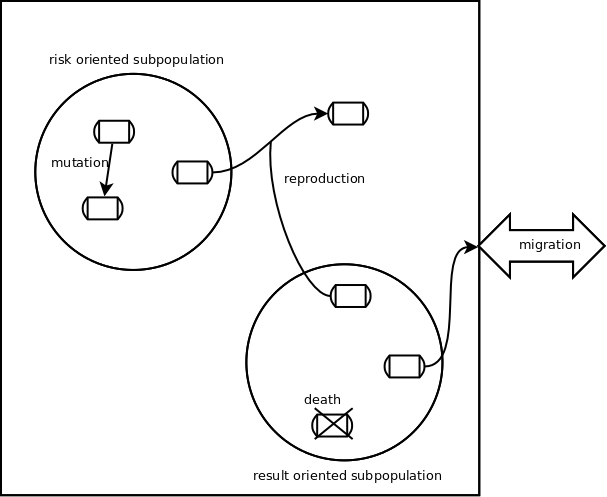
\includegraphics[scale=.35]{co-evol-2-sub.png}
	    \end{center}
	    \caption{Co-evolutionary system overview} 
	    \label{fig:co-evol}
	  \end{figure}

\subsection{Maintaining population diversity}

To sum up several mechanisms have been implemented to keep both subpopulations diverse:

\begin{itemize}
  \item crossover is allowed only between the fittest chromosomes from different subpopulations 
  \item mutations introducing random genetic change
  \item migration allows chromosomes to travel to different nodes  
\end{itemize}

\subsection{Pseudocode}

% \begin{algorithmic}
% 
% \STATE randomly INITIALISE both subpopulations (risk oriented and return oriented) 
% \FORALL{ $day$ }
%   \STATE EVALUATE each individual from both subpopulations
%   \STATE SELECT parents from both subpopulations
%   \STATE RECOMBINE pairs of parents to create offspring
%   \STATE MERGE existing subpopulations with newly created offspring
%   \STATE MUTATE part of the least fit population in both subpopulations
%   \STATE EVALUATE each individual from both subpopulations
%   \STATE EXTINCT part of the least fit population 
%   \RETURN non-dominated individual as a solution  
% \ENDFOR
% 
% \end{algorithmic}


\begin{algorithm}
  \SetKwData{returnOrientedSubpopulation}{returnOrientedSubpopulation}
  \SetKwData{riskOrientedSubpopulation}{riskOrientedSubpopulation}
  \SetKwData{parents}{parents}
  \SetKwData{offspring}{offspring}
  \SetKwData{population}{population}
  \SetKwData{mutants}{mutants}
  \SetKwFunction{evaluate}{evaluate}
  \SetKwFunction{initialise}{initialise}
  \SetKwFunction{selectParents}{selectParents}
  \SetKwFunction{recombine}{recombine}
  \SetKwFunction{merge}{merge}
  \SetKwFunction{mutateLeastFitIndividuals}{mutateLeastFitIndividuals}
  \SetKwFunction{extinctLeastFitIndividuals}{extinctLeastFitIndividuals}
  \SetKwInOut{Input}{input}\SetKwInOut{Output}{output}
 
  \BlankLine
  \initialise{\riskOrientedSubpopulation} \;
  \initialise{\returnOrientedSubpopulation} \;
  
  \ForEach{$day$}{ 

      \ForEach{$individual$ $\in$ \population}{
	  \evaluate($individual$)\;
      }
     
      \parents $\leftarrow$  \selectParents{\riskOrientedSubpopulation, \returnOrientedSubpopulation} \;
      \offspring $\leftarrow$ \recombine{\parents} \;
      \population  $\leftarrow$ \merge{\offspring, \riskOrientedSubpopulation, \returnOrientedSubpopulation} \;

      \mutateLeastFitIndividuals{\population} \;

      \ForEach{$individual$ $\in$ \population}{
	  \evaluate($individual$)\;
      }

      \extinctLeastFitIndividuals{\population} \;
      \Return{non-dominated solution} 
  }
  \caption{CoEMAS pseudocode}\label{coemas_pseudo}
\end{algorithm}

Contrary to GA, we are dealing with two populations (with different objectives) at once.
Apart from that, the pseudocode looks very similar.
Reproduction is only allowed between individuals from different subpopulations (which is a direct application of $restricted$ $mating$ method
 described in \ref{sec:population_diversity}).
To even further assure that populations remain diverse, we mutate part of the least fit individuals.
Extinction helps to control population size and get rid of useless individuals.
Non-dominated solution (in Pareto sense) is returned as a result.

\subsection{Class diagram}
\label{Co-evol-class-diagram}

Figure~\ref{fig:GA_UML} presents the UML class diagram of Genetic Algorithm.

\begin{figure}[ht]   
	    \begin{center}
	      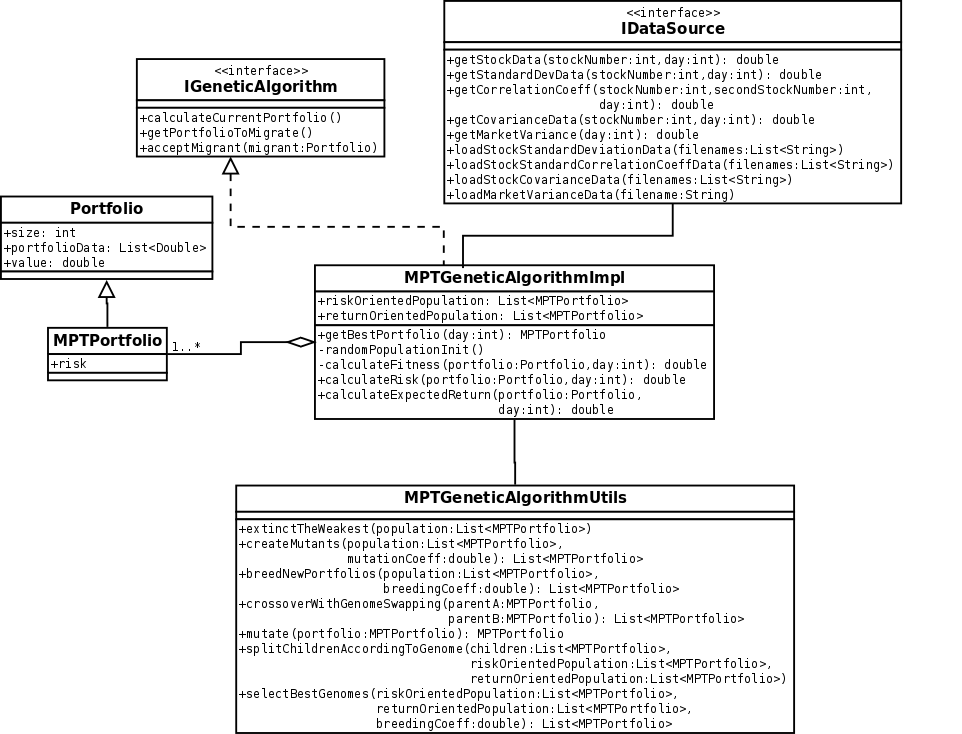
\includegraphics[scale=.35]{co-evol.png}
	    \end{center}
	    \caption{Class diagram of co-evolutionary system} 
	    \label{fig:GA_UML}
	  \end{figure}

\begin{description}
    \item [MPTPortfolio]
	This class represents the solution to the portfolio optimization problem - it contains portfolio composition as well as risk and expected return calculated
	due to CAPM formulas.
    \item [IDataSource]
	Any class implementing this interface would expose convenient access to all data (historical data as well as precomputed values of statistical functions)
	needed to calculate risk and expected return according to CAPM.
    \item [MPTGeneticAlgorithmImpl]
	Two subpopulations are present in this class as well as methods responsible for calculating risk and expected return according to CAPM. 
	    
    \item [MPTGeneticAlgorithmUtils]
	Utility class providing methods responsible for: mutating individuals, breeding new individuals, extincting the worst, etc. 
    
\end{description}




\section{Co-Evolutionary Multi-agent System - CoEMAS}

\subsection{Overview}

Co-evolutionary Multi-agent System (CoEMAS) is the most sophisticated system that has been implemented.
As described in \ref{sec:multi} and \ref{sec:co-evol} such systems need environment as well as a set of autonomous agents interacting with each other.
Potential solution to portfolio optimization problem is stored inside each agent.


\begin{figure}[ht]   
	    \begin{center}
	      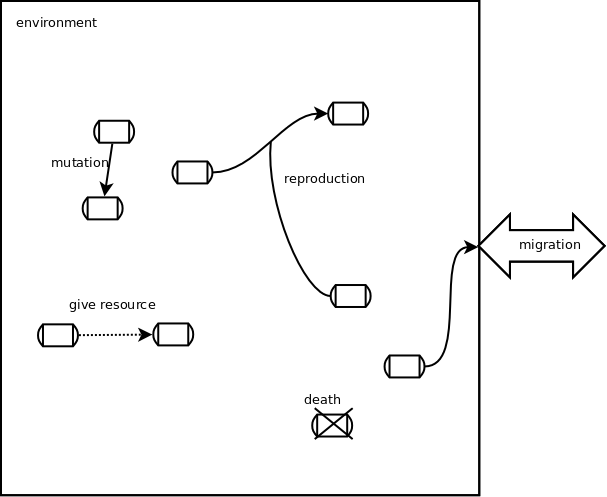
\includegraphics[scale=.38]{agent.png}
	    \end{center}
	    \caption{Overview of CoEMAS} 
	  \end{figure}

Contrary to \ref{sec:co-evol-sys} there are no subpopulations.
Instead of them we introduced individuals of two different species.
Each species focuses on different task:

\begin{itemize}
  \item species number 1 - tries to achieve the lowest risk possible
  \item species number 2 - tries to achieve the highest expected return possible
\end{itemize}

Risk as well as expected return is calculated due to Capital Asset Pricing Model (defined in \ref{CAPM}).

\subsection{Implemented actions}

Implemented actions that each agent can perform include (\ref{sec:CoEMAS}):

\begin{description}
  \item [death]
      if amount of resource that agent posses is lower than threshold value the agent dies
  \item [migration]
      agent is allowed to migrate but the probability of this action is low
  \item [reproduction]
      agents from different species are allowed to reproduce provided that they both exceed the minimum amount of resource allowing to reproduce
  \item [give/get]
      agent can get resource from other, dominated agent
  \item [recombination]
      agents produce offspring by the means of recombination
  \item [mutation]
      mutation introduces random change to potential solution, normalization of solution vector is then required 
  \item [seek]
      agents appropriate  to reproduction as well as get operation can be found thanks to this action
\end{description}

Interactions between agents are implemented in the following way:
\begin{itemize}
  \item co-evolution is implemented as a sequence of \emph{turns}
  \item in each \emph{turn} every agent perform its action (action to perform at any particular turn is chosen with some well defined probability, e.g. there is a 10\% chance that agent will try to find
	a partner to reproduce, 60\% chance that the agent will try to get some resource from dominated agent)
  \item when every agent performed some action the \emph{turn} ends and entire population of agents is checked whether some of them should die (not enough resource left after other agents got resource
	from it)
\end{itemize}


Each agent performs one of the above actions with some probability.

\subsection{Pseudocode}


% \STATE randomly INITIALISE agents of two different species (risk oriented and return oriented) 
% \FORALL{ $day$ }
% 
%   \FOR{$round = 1$ $to$  $number\_of\_rounds$}  
%       \FORALL{ $agent$ $\in$ population }
%   \STATE choose a profile for $agent$
%   \STATE $agent$ should act according to a selected profile  
%       \ENDFOR
%   \ENDFOR
%   \RETURN non-dominated agent as a solution  
% \ENDFOR


\begin{algorithm}
  \SetKwData{Profile}{profile}\SetKwData{This}{this}\SetKwData{Up}{up}
  \SetKwFunction{Union}{Union}\SetKwFunction{chooseProfile}{chooseProfile}
  \SetKwInOut{Input}{input}\SetKwInOut{Output}{output}
 
  \BlankLine
  \emph{randomly INITIALISE agents of two different species (risk oriented and return oriented)}\;
  \ForEach{$day$}{ 

    \For{$round\leftarrow 1$ \KwTo $number\_of\_rounds$}{\label{forins}
      \ForEach{$agent$ $\in$ population}{
      
      \Profile$\leftarrow$ \chooseProfile{}\;

      \If(){\Profile is $resource\_profile$ }{\label{lt}
        perform actions specified in $resource\_profile$ 
      }

      \If(){\Profile is $reproduction\_profile$ }{\label{lt}
        perform actions specified in $reproduction\_profile$ 
      }

      \If(){\Profile is $migration\_profile$ }{\label{lt}
        perform actions specified in $migration\_profile$ 
      }
      
    }
}
  }
  \caption{CoEMAS pseudocode}\label{coemas_pseudo}
\end{algorithm}


Profiles are chosen with following probabilities:
\begin{itemize}
  \item $resource$ $profile$ - with probability 0.6
  \item $reproduction$ $profile$ - with probability 0.2
  \item $migration$ $profile$ with probability 0.1
  \item $mutation$ $profile$ with probability 0.1
\end{itemize}

Similarly to \ref{sec:co-evol-sys}, mutation is used as a mean of maintaining population diversity.


\subsection{Class diagram}
\label{CoEMAS-class-diagram}

Figure~\ref{fig:coemas-uml} presents UML class diagram of CoEMAS.

\begin{figure}[ht]   
	    \begin{center}
	      \includegraphics[scale=.3]{CoEMAS-UML.png}
	    \end{center}
	    \caption{Class diagram of CoEMAS} 
	    \label{fig:coemas-uml}
	  \end{figure}

\begin{description}
  \item [Environment]
      aggregates all agents, responsible for population init at the start of algorithm and extinction of agents which resource level are too low, etc.
  \item [AgentUtils]
      utility class providing functions to Agent class
  \item [IAgent]
      interface specifying all methods that agent in CoEMAS should be capable of doing
  \item [Agent]
      implementation of agent that is autonomous and interact with other agents
  \item [IDataSource]
      provides easy access to historical data and computed statistical functions
 
\end{description}


%---------------------------------------------------------------------------

\section{Implementation details}
\label{sec:implDetails}


\subsection{Multi-agent running platform architecture}
\label{multi-agent}

%\clearpage
\begin{figure}[ht]
  \begin{center}
    \includegraphics[scale=.4]{agent_framework.png}
  \end{center}
  \caption{Deployment diagram of two Computing Nodes and Aggregation Node (in real situations more Computing Nodes are present)}
\end{figure}

Data Source as well as Computing Algorithm are created and injected to Computing Node(CN) by Spring. 
CNs send results of computations to Aggregating Node by JMS. 
Apart from that, JMS is used to provide migration capability to each CN.


\subsection{Precomputation of statistical functions}
\label{precompute}
Precomputation of statistical functions (like covariance, standard deviation etc.) from historical data is done by R scripts. 
Results are stored in files, later used as an input to other algorithms.
In order to provide easy and centralized access to historical data and precomputed statistical functions Data Source component has been introduced. 

\subsection{Data Source component}
\label{dataSource}

Data Source component aggregates all historical stock data as well as all precomputed statistical functions results from \ref{precompute}.   
Its interface enables access to all data it contains. Data Source is injected as a bean to other components by Spring.
They use it mainly as a source of data required by various algorithms.

\subsection{Computing Algorithm component}

Computing Algorithm component is responsible for carrying out all computations.
In order to function properly Data Source component as well as all configuration variables (like mutation coefficient etc.) has to be injected by Spring.
Apart from trend following algorithm, all the remaining approaches (CoEMAS (\ref{CoEMAS-class-diagram}), co-evolutionary (\ref{Co-evol-class-diagram}),
 genetic algorithm (\ref{gen-class-diagram})) can be injected to Computing Algorithm component so they can be run
 in a multi-agent system as a working horse of a Computing Node.


\subsection{Aggregating Node}

The sole purpose of Aggregating Node(AG) is to gather results from Computing Nodes(CN), choose the best non-dominated solution and write the results to file. 
Based on this file all charts are created and comparison of different algorithms is possible.
Communication between CNs and AG is provided by a single JMS queue (all CNs send results to one specific queue, AG consumes its content).


\subsection{Technologies used}

\begin{description}
  \item [R]
      Trend following algorithm has been implemented as an R script, historical data preprocessing.
  \item [Apache ActiveMQ]
      JMS implementation, provides communication between Computing Nodes and Aggregating Agent (\ref{multi-agent})
  \item [Java]
      Almost all algorithms are implemented in Java, Computing Nodes as well as Aggregating Node are in fact jar files.
      Java is an object oriented programming language that is portable, secure and robust.
      Java code is compiled to byte code interpeted by Java Virtual Machine. 
      It is very popular thanks to ease of application development. 
  \item [Inversion of Control]
	Inversion of Control (IoC) is an architectural pattern.
	It relies on concept of having an outside entity (usually it is called IoC container) that is responsible for wiring objects together. \cite{Spring} 
  \item [JMS]
	Java Message Service, it allows application to create, read, send and receive messages.
	Implementations of JMS provide reliable and asynchronous communication for distributed systems. 

  \item [Spring Framework]
      Inversion of Control container (configuration of application components and lifecycle management of Java objects), Messaging (simplifies the use of the JMS API) modules used.
  \item [Apache Maven]
      Used primarly for build automation.
  \item [JUnit]
      JUnit tests cover the most crucial functions of implemented algorithms.
  \item [git]
      Source Code Management tool.
  \item [bash scripts]
      Used for conveniently setting up and running test 
\end{description}

 